% questions.tex —— 1977 年·福建卷·理科 · 题目内容片段（无答案）
% 由 tools/generate_projects.py 依来源总账自 1977/1977_数学真题_福建理_试题.md 生成，勿手改（改源 MD 后重跑）


\gkpart{理科数学（福建卷）}

\begin{gktip}
\textbf{来源说明}：本题面依据固定源 PDF《1977 普通高等学校招生考试（福建卷理）》单页扫描逐题转录。源文件为 A3 单页题面，正式题为第 1—7 题，题面中“附加题”栏的第 8、9 题不计入正式题量。第 1 题含 10 个小问。第 5、第 6 和第 7 题存在源面参数异常或条件冲突，均按源页保留并在答案要点、解析正文和问题总账中标明。
\end{gktip}

\Needspace{0.4\textheight}
\begin{question}
\gkti{1}

\Needspace{5\baselineskip}
（1） 计算：

\nopagebreak[4]
\[
5-3\times\left[\left(-3\frac38\right)^{-\frac13}+1031\times\left(0.25-2^{-2}\right)\right]\div9^0
\]

\Needspace{5\baselineskip}
（2） 求下列式子的正负：

\nopagebreak[4]
\[
y=\frac{\cos160^\circ-\cos170^\circ}{\tan155^\circ}
\]

的值是正的还是负的？为什么？

\Needspace{5\baselineskip}
（3） 求函数

\nopagebreak[4]
\[
y=\frac{\lg(2-x)}{\sqrt{x}-1}
\]

的定义域。

（4） 如图，在梯形 $ABCD$ 中，$DM=MP=PA$，$MN\parallel PQ\parallel AB$，$DC=2\ \mathrm{cm}$，$AB=3.5\ \mathrm{cm}$，求 $MN$ 和 $PQ$ 的长。
\nopagebreak[4]
\begin{center}% 1977 年福建卷理科第 1(4) 题：梯形三等分平行线
\begin{tikzpicture}[scale=0.78]
  \coordinate (D) at (1.0,4.2);
  \coordinate (C) at (4.8,4.2);
  \coordinate (A) at (0,0);
  \coordinate (B) at (5.8,0);
  \coordinate (M) at ($(D)!1/3!(A)$);
  \coordinate (N) at ($(C)!1/3!(B)$);
  \coordinate (P) at ($(D)!2/3!(A)$);
  \coordinate (Q) at ($(C)!2/3!(B)$);
  \draw[thick] (D)--(C)--(B)--(A)--cycle;
  \draw[thick] (M)--(N);
  \draw[thick] (P)--(Q);
  \node[above left] at (D) {$D$};
  \node[above right] at (C) {$C$};
  \node[below left] at (A) {$A$};
  \node[below right] at (B) {$B$};
  \node[left] at (M) {$M$};
  \node[right] at (N) {$N$};
  \node[left] at (P) {$P$};
  \node[right] at (Q) {$Q$};
  \node[above] at (2.9,4.2) {$2$};
  \node[below] at (2.9,0) {$3.5$};
\end{tikzpicture}
\end{center}
\nopagebreak[4]
（5） 已知 $\lg3=0.4771$，$\lg x=-3.5229$，求 $x$。

\Needspace{5\baselineskip}
（6） 求

\nopagebreak[4]
\[
\lim_{x\to1}\frac{x-1}{x^2-3x+2}
\]

\Needspace{5\baselineskip}
（7） 解方程：

\nopagebreak[4]
\[
\sqrt{4x+1}-2x+1=0
\]

\Needspace{5\baselineskip}
（8） 化简：

\nopagebreak[4]
\[
\frac{a^{2n+1}-6a^{2n}+9a^{2n-1}}{a^{n+1}-4a^n+3a^{n-1}}
\]

（9） 求函数 $y=2-5x-3x^2$ 的极值。

（10） 画出下面 $V$ 形铁块的三视图（只要画草图）。
\nopagebreak[4]
\begin{center}% 1977 年福建卷理科第 1(10) 题：V 形铁块示意图
% 源卷只要求据图画三视图，未给尺寸；此处重绘结构关系，不虚构尺寸。
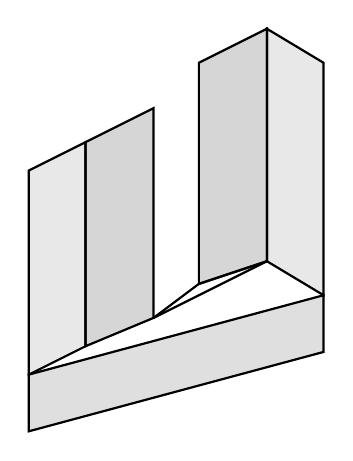
\begin{tikzpicture}[scale=0.72]
  \fill[gray!25] (0,0)--(5.2,1.4)--(5.2,2.4)--(0,1.0)--cycle;
  \draw[thick] (0,0)--(5.2,1.4)--(5.2,2.4)--(0,1.0)--cycle;
  \fill[gray!18] (0,1.0)--(0,4.6)--(1.0,5.1)--(1.0,1.5)--cycle;
  \fill[gray!32] (1.0,1.5)--(1.0,5.1)--(2.2,5.7)--(2.2,2.0)--cycle;
  \draw[thick] (0,1.0)--(0,4.6)--(1.0,5.1)--(1.0,1.5)--cycle;
  \draw[thick] (1.0,1.5)--(1.0,5.1)--(2.2,5.7)--(2.2,2.0)--cycle;
  \fill[gray!18] (5.2,2.4)--(5.2,6.5)--(4.2,7.1)--(4.2,3.0)--cycle;
  \fill[gray!32] (4.2,3.0)--(4.2,7.1)--(3.0,6.5)--(3.0,2.6)--cycle;
  \draw[thick] (5.2,2.4)--(5.2,6.5)--(4.2,7.1)--(4.2,3.0)--cycle;
  \draw[thick] (4.2,3.0)--(4.2,7.1)--(3.0,6.5)--(3.0,2.6)--cycle;
  \draw[thick] (2.2,2.0)--(3.0,2.6);
  \draw[thick] (2.2,2.0)--(4.2,3.0);
  \draw[thick] (3.0,2.6)--(4.2,3.0);
  \draw[dashed] (2.2,2.0)--(2.2,5.7);
  \draw[dashed] (3.0,2.6)--(3.0,6.5);
\end{tikzpicture}
\end{center}
\nopagebreak[4]
\end{question}
\begin{question}
\gkti{2}

\Needspace{5\baselineskip}
（1） 解不等式：

\nopagebreak[4]
\[
\frac{x^2-x-6}{x^2+2x+2}<0
\]

\Needspace{5\baselineskip}
（2） 证明：

\nopagebreak[4]
\[
\frac{2\cos\theta-\sin2\theta}{2\cos\theta+\sin2\theta}
=\tan^2\left(\frac{90^\circ-\theta}{2}\right)
\]

（3） 某中学革命师生自己动手油漆一个直径为 $1.2\ \mathrm m$ 的地球仪，如果每平方米面积需要油漆 $150$ 克，问共需油漆多少克？（答案保留整数。）

（4） 某农机厂开展“工业学大庆”运动，在十月份生产拖拉机 $1000$ 台。这样，一月至十月的产量恰好完成全年生产任务。工人同志为了加速农业机械化，计划在年底前再生产 $2310$ 台，求十一月、十二月份平均每月增长率。

\end{question}
\begin{question}
\gkti{3}在半径为 $R$ 的圆内接正六边形内，依次连接各边的中点，得一正六边形；又在这一正六边形内，再依次连接各边的中点，又得一正六边形，这样无限地继续下去，求：

（1） 前 $n$ 个正六边形的周长之和 $S_n$；

（2） 所有这些正六边形的周长之和 $S$。

\end{question}
\begin{question}
\gkti{4}动点 $P(x,y)$ 到两定点 $A(-3,0)$ 和 $B(3,0)$ 的距离的比等于 $2$，求动点 $P$ 的轨迹方程，并说明这轨迹是什么图形。

\Needspace{0.4\textheight}
\end{question}
\begin{question}
\gkti{5}某大队在农田基本建设的规划中，要测定被障碍物隔开的两点 $A\text{、}P$ 之间的距离，他们土法上马，在障碍物的两侧选取两点 $B$ 和 $C$（如图），测得 $AB=AC=50\ \mathrm m$，$\angle BAC=60^\circ$，$\angle ABP=120^\circ$，$\angle ACP=135^\circ$，求 $A$ 和 $P$ 之间的距离。（答案可用最简根式表示。）
\nopagebreak[4]
\begin{center}% 1977 年福建卷理科第 5 题：障碍物两侧测距示意图
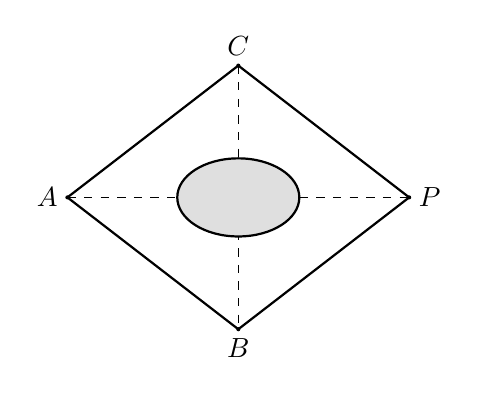
\begin{tikzpicture}[scale=0.62]
  \coordinate (A) at (0,0);
  \coordinate (P) at (7.0,0);
  \coordinate (C) at (3.5,2.7);
  \coordinate (B) at (3.5,-2.7);
  \draw[thick] (A)--(C)--(P)--(B)--cycle;
  \draw[dashed] (A)--(P);
  \draw[dashed] (C)--(B);
  \fill[gray!25] (3.5,0) ellipse (1.25 and 0.8);
  \draw[thick] (3.5,0) ellipse (1.25 and 0.8);
  \fill (A) circle (1.2pt) node[left] {$A$};
  \fill (P) circle (1.2pt) node[right] {$P$};
  \fill (C) circle (1.2pt) node[above] {$C$};
  \fill (B) circle (1.2pt) node[below] {$B$};
\end{tikzpicture}
\end{center}
\nopagebreak[4]
\end{question}
\begin{question}
\gkti{6}已知双曲线

\nopagebreak[4]
\[
\frac{x^2}{24\alpha}-\frac{y^2}{16\cot\alpha}=1\quad(\alpha\text{ \text{为锐角}})
\]

和圆 $(x-m)^2+y^2=r^2$ 相切于点 $A(4\sqrt3,4)$，求 $\alpha\text{、}m\text{、}r$ 的值。

\end{question}
\begin{question}
\gkti{7}设数列 $1,2,4,\ldots$ 前 $n$ 项和是

\nopagebreak[4]
\[
S_n=a+bn+cn^2+dn^3
\]

求这数列的通项 $a_n$ 的公式，并确定 $a,b,c,d$ 的值。

\begin{gktip}
\Needspace{0.25\textheight}
\textbf{附加题}
\end{gktip}

\Needspace{5\baselineskip}
\textbf{附加题 8．} 求函数

\nopagebreak[4]
\[
y=\mathrm e^{-2x}\sin\left(5x+\frac\pi4\right)
\]

的导数。

\Needspace{5\baselineskip}
\textbf{附加题 9．} 求定积分：

\nopagebreak[4]
\[
\int_0^1\left(x\mathrm e^{x^2}+x^2\mathrm e^{2x}\right)\,\mathrm dx
\]

\end{question}